\documentclass[11pt]{article}
\usepackage[T1]{fontenc}
\usepackage{lmodern}
\usepackage[a4paper,margin=1in]{geometry}
\usepackage{amsmath,amssymb,amsthm,mathtools}
\usepackage{booktabs}
\usepackage{graphicx}
\usepackage{float}
\usepackage[hidelinks]{hyperref}

\hypersetup{
  pdftitle={From Singleton to Set Retention in KL Contraction of Finite Markov Chains},
  pdfauthor={Saurav Jadhav},
  pdfsubject={Kullback--Leibler contraction and set-conditioned witnesses}
}

\newtheorem{theorem}{Theorem}[section]
\newtheorem{proposition}[theorem]{Proposition}
\newtheorem{corollary}[theorem]{Corollary}
\newtheorem{lemma}[theorem]{Lemma}
\newtheorem{remark}[theorem]{Remark}
\newtheorem{definition}[theorem]{Definition}

\newcommand{\KL}{D_{\mathrm{KL}}}
\newcommand{\etaKL}{\eta_{\mathrm{KL}}}
\newcommand{\etaStat}{\eta_{\mathrm{KL}}(\pi,P)}
\newcommand{\Mone}{M_1}
\newcommand{\Lone}{L_1}
\newcommand{\Mset}{M_{\mathrm{set}}}
\newcommand{\E}{\mathbb{E}}
\newcommand{\MI}{I}
\newcommand{\Ent}{\mathrm{Ent}}
\newcommand{\kl}{\operatorname{kl}}

\title{From Singleton to Set Retention in KL Contraction\\
of Finite Markov Chains}
\author{
  Saurav Jadhav\thanks{Independent Researcher, Pune, India.
    Email: sauravjadhav698@gmail.com}
}
\date{}

\begin{document}

\maketitle

\begin{abstract}
For a finite Markov kernel \(P\) with full-support stationary law \(\pi\),
the fixed-reference Kullback--Leibler contraction coefficient optimizes over
all initial distributions.  Point masses give transparent feasible tests:
\[
  r(x)=\frac{\KL(P(x,\cdot)\|\pi)}{\log(1/\pi(x))}.
\]
We organize these singleton tests into a stationary profile with envelope
\(\Mone=\max_x r(x)\).  When \(\Mone>0\), its survival curve and scalar
localization index are
\(F_1(t)=\pi\{r\ge t\Mone\}\) and
\(\Lone=\E_\pi r/\Mone\).  The main question is whether a small set of
high-retention states also controls the full contraction coefficient.

The answer is negative without structural assumptions.  The standard
KL chain rule yields an exact decomposition in which spreading an input law
creates entropy while distinguishable transition rows incur a
mutual-information penalty.  Exploiting identical rows, we construct
strictly positive reversible kernels for which
\[
  \Lone\longrightarrow0,\qquad
  \Mone\longrightarrow0,\qquad
  \etaKL(\pi,P)\longrightarrow1,
  \qquad
  \etaKL(\pi,P)/\Mone\longrightarrow\infty .
\]
Thus singleton localization does not provide a uniform approximation to,
or control of, global KL contraction.

This failure motivates a collective diagnostic.  For every nonempty proper
set \(A\), let
\[
  R(A)=
  \frac{\KL(\pi(\cdot\mid A)P\|\pi)}{\log(1/\pi(A))},
  \qquad
  \Mset=\max_A R(A).
\]
Then \(\Mone\le\Mset\le\etaKL(\pi,P)\).  A binary data-processing argument
shows, uniformly for \(\pi(A)\le1/2\), that small one-step escape probability
forces \(R(A)\) close to one, including for balanced bottlenecks where the corresponding
singleton bound can vanish.  We also prove exact preservation of
clone-saturated set tests under proportional state splitting, record selected spectral comparisons, and
work out analytic examples.  The resulting picture separates a
statewise diagnostic from a collective obstruction without mistaking
either for the full variational problem.
\end{abstract}

\noindent\textbf{Keywords:}
strong data processing inequalities, Kullback--Leibler divergence,
Markov chains, mutual information, conductance, state aggregation.


\section{Introduction}
\label{sec:intro}

\subsection{Can a cloud of states remember more than any one state?}

Consider a finite Markov kernel \(P\) with stationary distribution \(\pi\).
Its fixed-reference KL contraction coefficient is
\begin{equation}
  \etaStat
  :=
  \sup_{\mu\ne\pi}
  \frac{\KL(\mu P\|\pi)}{\KL(\mu\|\pi)}.
  \label{eq:eta-intro}
\end{equation}
It measures the largest fraction of relative entropy to stationarity that
can survive one step.  The optimization ranges over an entire probability
simplex.  A first attempt is therefore to test its vertices:
\[
  \mu=\delta_x
  \quad\Longrightarrow\quad
  r(x)
  =
  \frac{\KL(P(x,\cdot)\|\pi)}{\log(1/\pi(x))}.
\]
This produces one number per state rather than one opaque supremum.

The statewise view raises a concrete question.  Is slow information loss
caused by one exceptional transition row, by a diffuse collection of
individually bad states, or by a collection that becomes informative only
when treated as a whole?  Put differently: can a cloud of states retain
almost all of its KL divergence even though no single state does?

The distinction matters because an initial law can exploit multiplicity.
Spreading mass over several states increases its entropy, while identical
transition rows reveal nothing about which of those states was selected.
The denominator in \eqref{eq:eta-intro} can then fall without a corresponding
information penalty after one step.  This mechanism is invisible to a
profile containing only singleton tests.

\subsection{Main results and the paper's claim}

We first organize the singleton witnesses into an envelope and, when
\(\Mone>0\), a normalized curve and scalar index:
\[
  \Mone=\max_x r(x),\qquad
  F_1(t)=\pi\{x:r(x)\ge t\Mone\},\qquad
  \Lone=\frac{\E_\pi r}{\Mone}
       =\int_0^1 F_1(t)\,dt .
\]
The curve \(F_1\), rather than the scalar \(\Lone\), is the primary
localization object.  It records how much stationary mass lies above every
relative retention threshold.  The scalar \(\Lone\) is only its area.

The central identity is the standard Jensen-gap decomposition
\[
  \KL(\mu P\|\pi)
  =
  \sum_x\mu(x)\KL(P(x,\cdot)\|\pi)-I_\mu(X;Y).
\]
Combining it with \(r(x)\le\Mone\) gives an exact criterion for an input law
to beat every point mass.  The identity itself is classical; its role here
is to expose the precise failure mode of the singleton envelope.

Our strongest negative result is an unbounded separation theorem.  There
exist finite, strictly positive, reversible kernels for which
\[
  \Lone\to0,\qquad \Mone\to0,\qquad
  \etaStat\to1,\qquad \etaStat/\Mone\to\infty.
\]
The near-extremizing law is the stationary distribution conditioned on a
small set of states with identical rows.  This result rules out any
interpretation of \(\Lone\) as evidence that point masses are nearly
optimal, even when the high-retention singleton set has vanishing
stationary mass.

The same construction suggests the repair.  We retain conditional
stationary laws as a first collective layer:
\[
  R(A)=
  \frac{\KL(\pi(\cdot\mid A)P\|\pi)}{\log(1/\pi(A))}.
\]
The resulting envelope satisfies
\(\Mone\le\Mset\le\etaStat\), contains the class-conditioned witness
\(R(C)\) for every identical-row class, and
preserves every original set test under a natural proportional splitting
of states.  It also has a
direct bottleneck interpretation.  If \(h(A)\) is the one-step escape
probability from \(A\) under \(\pi(\cdot\mid A)\), then
\[
  R(A)\ge
  \frac{\kl(1-h(A)\|\pi(A))}{\log(1/\pi(A))}.
\]
For fixed \(\pi(A)\), the right-hand side tends to one as \(h(A)\to0\).
Unlike the induced singleton bound, this remains informative for balanced
cuts.

This is a limitation and diagnostic note centered on one obstruction.  The
main mathematical contribution is the unbounded separation theorem.  We
additionally propose the singleton-to-set organization as a diagnostic for
the missing collective layer.  Point-mass tests, fixed-reference
SDPIs, the Jensen-gap identity, and quadratic near-stationary contraction
are standard tools rather than novelty claims.

\subsection{Relation to prior work}
\label{sec:related}

\paragraph{Fixed-reference contraction.}
Strong data-processing inequalities distinguish a channel coefficient,
which optimizes over two input laws, from the fixed-reference coefficient
in \eqref{eq:eta-intro}; see Raginsky~\cite{Raginsky2016} and
Polyanskiy--Wu~\cite{PolyanskiyWu2017}.  The coefficient in
\eqref{eq:eta-intro} is the discrete-time
fixed-reference SDPI coefficient, or retained fraction; its complement
\(1-\etaStat\) is the full-step entropy contraction coefficient used in the
Markov-chain literature.  Caputo--Chen--Gu--Polyanskiy~\cite{CaputoEtAl2025} compare this full-step constant
with half-step and continuous-time notions, construct sharp separations,
and analyze extremizers.  Earlier general results on relative entropy under
stochastic matrices include Cohen et al.~\cite{CohenEtAl1993}.  Accordingly,
we restrict attention to the discrete-time, fixed-reference problem.

\paragraph{Point inputs and stationary row divergence.}
Point masses are standard feasible tests for a fixed-reference SDPI; their
use is not new.  For the nonlazy complete-graph walk on \(K_n\), \(n\ge3\),
the fixed-entropy reduction and strict endpoint argument of
Gu--Polyanskiy~\cite[Proposition~18 and Section~5.2]{GuPolyanskiy2023}
show that point masses are in fact the only extremizers.  Choi--Hird--Wang
\cite{ChoiHirdWang2025} use
\[
  D_{\mathrm{KL}}^\pi(P\|\Pi)
  =\sum_x\pi(x)\KL(P(x,\cdot)\|\pi),
  \qquad \Pi(x,\cdot)=\pi,
\]
as a weighted kernel divergence.  Under stationarity this quantity equals
\(I(X_0;X_1)\).  Our profile retains the statewise summands and normalizes
each by the entropy of the corresponding point mass.

\paragraph{Mixtures and information geometry.}
The gap between an average KL divergence and the divergence of the average
is generalized Jensen--Shannon divergence, equivalently the KL case of
Bregman information; see Lin~\cite{Lin1991} and
Banerjee--Merugu--Dhillon--Ghosh~\cite{BanerjeeEtAl2005}.  We use this
standard identity to compare entropy inflation with the information
revealed by distinct rows.

\paragraph{Sets, bottlenecks, and representation.}
Conditioned stationary laws and low-boundary sets are classical in
conductance and evolving-set arguments
\cite{LawlerSokal1988,MorrisPeres2005,LevinPeres2017,Montenegro2007}.
We do not claim that testing such laws is new.  The point here is to retain
their exact fixed-reference KL ratios in the same diagnostic hierarchy as
the singleton tests.  State aggregation and entropy under lumping have a
separate literature; see Geiger--Temmel~\cite{GeigerTemmel2014}.  Our
splitting result concerns one precise refinement operation and should not
be read as invariance under arbitrary lumping.

\paragraph{A distinct use of the word local.}
Daeijavad--Asoodeh~\cite{DaeijavadAsoodeh2026} study global and local
contraction for MCMC under \(E_\gamma\)-divergence, where the local
coefficient is restricted to a high-probability core and paired with a
tail profile.  That operational notion is mathematically distinct from
the statewise, fixed-reference KL witnesses studied here.  To avoid a
collision of terminology, we use \emph{singleton retention} for \(r(x)\)
and \emph{quadratic near-stationary} for infinitesimal perturbations of
\(\pi\).

\subsection{Organization}

Section~\ref{sec:singleton} defines the singleton profile and derives the
mixture decomposition.  Section~\ref{sec:multiplicity} proves the
unbounded separation theorem.  Section~\ref{sec:set} introduces
set-conditioned retention, proves the splitting and bottleneck results,
and recovers the weaker singleton Cheeger bound as a corollary.
Section~\ref{sec:spectral} distinguishes singleton, stationary-average, and
near-stationary behavior.  Section~\ref{sec:examples} gives analytic examples
and a profile figure.
Section~\ref{sec:conclusion} states the limitations and the structural
questions left open.  Appendix~\ref{app:spectral} contains the longer
\(\chi^2\)-spectral comparison and a supplementary three-state example.


\section{Singleton retention and mixtures}
\label{sec:singleton}

\subsection{Setup and the singleton profile}

Let \(S\) be a finite set with \(|S|=n\ge2\).  Throughout, \(P\) is a
Markov kernel on \(S\), and \(\pi\) is a full-support stationary law:
\[
  \pi(x)>0\quad(x\in S),\qquad \pi P=\pi.
\]
Irreducibility guarantees such a law is unique, but uniqueness is not
needed for the algebra below.  All logarithms are natural.  For probability
laws \(\mu,\nu\) on \(S\),
\[
  \KL(\mu\|\nu)
  =\sum_{x\in S}\mu(x)\log\frac{\mu(x)}{\nu(x)},
\]
with the usual convention \(0\log0=0\).  Since \(\pi\) has full support,
all divergences to \(\pi\) are finite.  By data processing
\cite{CoverThomas2006}, stationarity gives
\[
  0\le
  \frac{\KL(\mu P\|\pi)}{\KL(\mu\|\pi)}
  \le1
  \qquad(\mu\ne\pi).
\]

\begin{definition}[Singleton retention profile]
\label{def:singleton-profile}
For \(x\in S\), define
\[
  r(x)
  :=
  \frac{\KL(P(x,\cdot)\|\pi)}{\log(1/\pi(x))}.
\]
Its stationary mean and envelope are
\[
  \bar r_\pi:=\sum_x\pi(x)r(x),
  \qquad
  \Mone:=\max_x r(x).
\]
When \(\Mone>0\), define the normalized survival curve and its scalar
localization index by
\[
  F_1(t):=\pi\{x:r(x)\ge t\Mone\},
  \quad 0\le t\le1,
  \qquad
  \Lone:=\frac{\bar r_\pi}{\Mone}.
\]
\end{definition}

If \(\Mone=0\), then every row equals \(\pi\), so \(P=\Pi\) and
\(\etaStat=0\).  In that degenerate case \(F_1\) and \(\Lone\) are left
undefined; declaring such a chain maximally localized or delocalized would
attach geometry to the absence of any obstruction.

\begin{proposition}[Singleton hierarchy and profile area]
\label{prop:singleton-hierarchy}
For every stationary pair \((\pi,P)\),
\[
  0\le \bar r_\pi\le\Mone\le\etaStat\le1.
\]
If \(\Mone>0\), then
\[
  \Lone=\int_0^1F_1(t)\,dt,
  \qquad
  F_1(t)\le \min\!\left\{1,\frac{\Lone}{t}\right\}
  \quad(0<t\le1).
\]
\end{proposition}

\begin{proof}
For each \(x\), the law \(\delta_x\) is an admissible test in
\eqref{eq:eta-intro}, and
\[
  \KL(\delta_x\|\pi)=\log(1/\pi(x)),\qquad
  \KL(\delta_xP\|\pi)=\KL(P(x,\cdot)\|\pi).
\]
Hence \(0\le r(x)\le\etaStat\le1\).  Averaging and maximizing prove the
hierarchy.  The layer-cake identity applied to \(r(X)/\Mone\in[0,1]\)
gives the integral formula.  Markov's inequality gives the tail bound.
\end{proof}

The curve \(F_1\) contains strictly more information than \(\Lone\).
Two profiles with the same area can place that area at very different
thresholds.  Conversely, \(\Lone\ll1\) means only that the high-retention
singletons have small stationary mass.  It does not bound their cardinality,
their row multiplicity, or the performance of mixtures supported on them.

\begin{proposition}[Uniform stationary law]
\label{prop:uniform-entropy}
If \(\pi\) is uniform on \(S\), then
\[
  r(x)=1-\frac{H(P(x,\cdot))}{\log n},
  \qquad
  \Mone=1-\frac{\min_x H(P(x,\cdot))}{\log n},
\]
where \(H(q)=-\sum_yq(y)\log q(y)\).
\end{proposition}

\begin{proof}
For uniform \(\pi\),
\(\KL(P(x,\cdot)\|\pi)=\log n-H(P(x,\cdot))\), while
\(\log(1/\pi(x))=\log n\).
\end{proof}

\subsection{The exact mixture penalty}

Let \(X\sim\mu\) and, conditionally on \(X=x\), let
\(Y\sim P(x,\cdot)\).  The output law is \(\mu P\), and
\[
  I_\mu(X;Y)
  :=\sum_x\mu(x)\KL(P(x,\cdot)\|\mu P).
\]
This is the generalized Jensen--Shannon divergence of the rows under
weights \(\mu\).

\begin{theorem}[Mixture identity and singleton envelope]
\label{thm:mixture-identity}
For every probability law \(\mu\) on \(S\),
\begin{equation}
  \KL(\mu P\|\pi)
  =
  \sum_x\mu(x)\KL(P(x,\cdot)\|\pi)-I_\mu(X;Y).
  \label{eq:mixture-identity}
\end{equation}
Consequently, for every \(\mu\ne\pi\),
\begin{align}
  \frac{\KL(\mu P\|\pi)}{\KL(\mu\|\pi)}
  &=
  \frac{\sum_x\mu(x)r(x)\log(1/\pi(x))-I_\mu(X;Y)}
       {\KL(\mu\|\pi)},                                      \label{eq:exact-envelope}\\
  \frac{\KL(\mu P\|\pi)}{\KL(\mu\|\pi)}-\Mone
  &=
  \frac{
    \Mone H(\mu)-I_\mu(X;Y)
    -\sum_x\mu(x)(\Mone-r(x))\log(1/\pi(x))
  }{\KL(\mu\|\pi)}.                                         \label{eq:beat-singleton}
\end{align}
In particular, \(\mu\) beats every singleton test if and only if
\[
  \Mone H(\mu)>
  I_\mu(X;Y)
  +\sum_x\mu(x)(\Mone-r(x))\log(1/\pi(x)).
\]
\end{theorem}

\begin{proof}
The KL chain rule gives
\[
  \sum_x\mu(x)\KL(P(x,\cdot)\|\pi)
  =
  \sum_x\mu(x)\KL(P(x,\cdot)\|\mu P)
  +\KL(\mu P\|\pi),
\]
which is \eqref{eq:mixture-identity}.  Substitute the definition of
\(r(x)\) to obtain \eqref{eq:exact-envelope}.  Finally,
\[
  \sum_x\mu(x)\log\frac1{\pi(x)}
  =\KL(\mu\|\pi)+H(\mu).
\]
Add and subtract
\(\Mone\sum_x\mu(x)\log(1/\pi(x))\), and then subtract
\(\Mone\KL(\mu\|\pi)\), to obtain \eqref{eq:beat-singleton}.
\end{proof}

Equation~\eqref{eq:beat-singleton} separates three effects.  Spreading
\(\mu\) creates the entropy term \(\Mone H(\mu)\).  Distinguishable rows
create the mutual-information penalty \(I_\mu(X;Y)\).  Placing mass below
the singleton envelope creates the row-deficit penalty.  Near stationarity
the terms may cancel at second order; the expression is an identity, not
a standalone upper bound on \(\etaStat-\Mone\).

\begin{proposition}[Identical-row reduction]
\label{prop:row-equivalence}
Partition \(S\) into equivalence classes under
\[
  x\sim x'
  \quad\Longleftrightarrow\quad
  P(x,\cdot)=P(x',\cdot),
\]
and let \(J\) be the class containing \(X\).  Then
\[
  I_\mu(X;Y)=I_\mu(J;Y)
\]
for every input law \(\mu\).
\end{proposition}

\begin{proof}
The conditional law of \(Y\) given \(X=x\) depends on \(x\) only through
\(J\).  Thus \(X\to J\to Y\), \(J\) is a function of \(X\), and
\(I(X;Y)=I(J;Y)+I(X;Y\mid J)=I(J;Y)\).
\end{proof}

Randomization within one identical-row class can therefore increase
\(H(\mu)\) without increasing the mutual-information penalty.  This is the
mechanism behind the next section.


\section{Multiplicity makes singleton tests arbitrarily bad}
\label{sec:multiplicity}

The following theorem is the main limitation result: the singleton envelope
and localization index vanish simultaneously while the global coefficient
tends to one.

\begin{theorem}[Unbounded failure of singleton localization]
\label{thm:unbounded-separation}
There exists a sequence of finite, strictly positive, reversible Markov
kernels \((\pi_m,P_m)\) such that
\[
  \Lone(P_m)\longrightarrow0,\qquad
  \Mone(P_m)\longrightarrow0,\qquad
  \etaKL(\pi_m,P_m)\longrightarrow1,
\]
and hence
\[
  \frac{\etaKL(\pi_m,P_m)}{\Mone(P_m)}
  \longrightarrow\infty.
\]
Moreover, for each \(m\) the near-unit contraction ratio is witnessed by
\(\pi_m(\cdot\mid A_m)\), where all states in \(A_m\) have the same
transition row.
\end{theorem}

\begin{proof}
The construction gives a small total stationary mass \(\varepsilon\) to a
block \(A\) containing many states with identical rows.  A large spectator
block \(B\) dilutes its own singleton retention through the state count
\(N\), while \(\delta>0\) keeps every transition positive and can later be
sent toward the desired block limit.  Formally, fix
\(\varepsilon\in(0,1/2)\), integers \(k,N\ge1\), and
\(\delta\in(0,1)\).  Let \(S=A\sqcup B\), with \(|A|=k\) and
\(|B|=N\), and set
\[
  \pi(a)=\frac{\varepsilon}{k}\quad(a\in A),
  \qquad
  \pi(b)=\frac{1-\varepsilon}{N}\quad(b\in B).
\]
For \(a\in A\), define
\[
  P(a,x)=
  \begin{cases}
    (1-\delta)/k,&x\in A,\\
    \delta/N,&x\in B,
  \end{cases}
\]
and, for \(b\in B\), define
\[
  P(b,x)=
  \begin{cases}
    \dfrac{\varepsilon\delta}{k(1-\varepsilon)},&x\in A,\\[6pt]
    \dfrac{1-\varepsilon-\varepsilon\delta}{N(1-\varepsilon)},&x\in B.
  \end{cases}
\]
Every entry is positive because
\(1-\varepsilon-\varepsilon\delta>1-2\varepsilon>0\).  The \(A\)-rows
plainly sum to one, while each \(B\)-row has total mass
\[
  \frac{\varepsilon\delta}{1-\varepsilon}
  +\frac{1-\varepsilon-\varepsilon\delta}{1-\varepsilon}
  =1.
\]
Detailed balance holds
across the two blocks because
\[
  \pi(a)P(a,b)
  =\frac{\varepsilon\delta}{kN}
  =\pi(b)P(b,a).
\]
Symmetry inside each block completes the reversibility check.

Rows are constant on each block.  Define
\[
  d_A(\delta)
  :=
  (1-\delta)\log\frac{1-\delta}{\varepsilon}
  +\delta\log\frac{\delta}{1-\varepsilon}
\]
and
\[
  \alpha_\delta:=\frac{\varepsilon\delta}{1-\varepsilon},
  \qquad
  d_B(\delta)
  :=
  \alpha_\delta\log\frac{\alpha_\delta}{\varepsilon}
  +(1-\alpha_\delta)
    \log\frac{1-\alpha_\delta}{1-\varepsilon}.
\]
Since both \(P\) and \(\pi\) are uniform within each block, binary
aggregation loses no divergence.  Thus
\[
  r_A(\delta)=\frac{d_A(\delta)}{\log(k/\varepsilon)},
  \qquad
  r_B(\delta)=\frac{d_B(\delta)}{\log(N/(1-\varepsilon))}.
\]
As \(\delta\downarrow0\),
\begin{align*}
  r_A(\delta)&\longrightarrow
  a_{\varepsilon,k}
  :=\frac{\log(1/\varepsilon)}{\log(k/\varepsilon)},\\
  r_B(\delta)&\longrightarrow
  b_{\varepsilon,N}
  :=\frac{\log(1/(1-\varepsilon))}
          {\log(N/(1-\varepsilon))}.
\end{align*}
For fixed \(\varepsilon\), \(b_{\varepsilon,N}\to0\) as \(N\to\infty\).

Now take \(\mu=\pi(\cdot\mid A)\).  Because the rows on \(A\) are
identical,
\[
  \mu P=P(a,\cdot)\quad(a\in A),
  \qquad
  \KL(\mu\|\pi)=\log(1/\varepsilon),
\]
and therefore
\begin{equation}
  \frac{\KL(\mu P\|\pi)}{\KL(\mu\|\pi)}
  =\frac{d_A(\delta)}{\log(1/\varepsilon)}
  \longrightarrow1
  \quad(\delta\downarrow0).
  \label{eq:collective-witness}
\end{equation}

It remains to select one diagonal sequence.  For integers \(m\ge3\), set
\[
  \varepsilon_m=e^{-m},
  \qquad
  k_m=\left\lceil e^{m^2}\right\rceil,
  \qquad
  a_m:=a_{\varepsilon_m,k_m}
  =\frac{m}{m+\log k_m}.
\]
Then \(a_m\sim1/(m+1)\).  Choose \(N_m\) large enough that
\[
  b_{\varepsilon_m,N_m}\le\frac{a_m}{m}.
\]
By continuity in \(\delta\), choose \(\delta_m>0\) so small that
\[
  a_m\Bigl(1-\frac1m\Bigr)
  \le r_A(\delta_m)
  \le a_m\Bigl(1+\frac1m\Bigr),
  \qquad
  r_B(\delta_m)\le\frac{2a_m}{m},
\]
and the ratio in \eqref{eq:collective-witness} is at least \(1-1/m\).
Let \((\pi_m,P_m)\) be the stationary pair obtained from these parameter
choices.  For all large \(m\),
\[
  a_m\Bigl(1-\frac1m\Bigr)
  \le\Mone(P_m)
  \le a_m\Bigl(1+\frac1m\Bigr),
\]
so \(\Mone(P_m)\to0\).  Moreover,
\begin{align*}
  \Lone(P_m)
  &=
  \frac{\varepsilon_m r_A(\delta_m)
        +(1-\varepsilon_m)r_B(\delta_m)}
       {\Mone(P_m)}\\
  &\le
  \varepsilon_m+
  \frac{r_B(\delta_m)}{r_A(\delta_m)}
  \le
  e^{-m}+\frac{2}{m-1}
  \longrightarrow0.
\end{align*}
Finally,
\[
  1\ge\etaKL(\pi_m,P_m)\ge1-\frac1m,
\]
so the coefficient tends to one.  Combining this with the upper estimate
on \(\Mone(P_m)\) gives
\[
  \frac{\etaKL(\pi_m,P_m)}{\Mone(P_m)}
  \ge
  \frac{1-1/m}{a_m(1+1/m)}
  \longrightarrow\infty.
\]
\end{proof}

The theorem is intentionally sensitive to the finite-state representation:
without assumptions controlling row multiplicity or distinguishability,
there is no dimension-free constant \(C\) for which
\(\etaKL(\pi,P)\le C\Mone(P)\) holds uniformly over all finite stationary
pairs.  In fact, for fixed \((\varepsilon,\delta)\), the construction is the
proportional splitting of a reversible two-state block kernel with stationary
law \((\varepsilon,1-\varepsilon)\) into \(k\) and \(N\) clones.  The block
dynamics are unchanged; what changes is the point-mass normalization.

The obstruction is not a rare exceptional state.  It is the multiplicity
of an informationally indistinguishable class.  The statistic \(\Lone\)
correctly reports that high singleton retention occupies little stationary
mass; it cannot report that conditioning on the entire class removes
\(\log k\) units from the input divergence while leaving the output
unchanged.


\section{Set-conditioned retention}
\label{sec:set}

\subsection{The first collective layer}

\begin{definition}[Set-conditioned KL retention]
\label{def:set-retention}
For every nonempty proper set \(A\subsetneq S\), write
\[
  \pi_A:=\pi(\cdot\mid A)
\]
and define
\[
  R(A)
  :=
  \frac{\KL(\pi_AP\|\pi)}{\KL(\pi_A\|\pi)}
  =
  \frac{\KL(\pi_AP\|\pi)}{\log(1/\pi(A))}.
\]
The set-retention envelope is
\[
  \Mset:=
  \max_{\varnothing\ne A\subsetneq S}R(A).
\]
\end{definition}

The exclusion \(A=S\) is essential because the denominator then vanishes.
We do not restrict to \(\pi(A)\le1/2\): doing so would discard singleton
tests for states of mass greater than one half.

\begin{proposition}[Singleton--set--global hierarchy]
\label{prop:set-hierarchy}
For every stationary pair \((\pi,P)\),
\[
  0\le R(A)\le1
  \quad(\varnothing\ne A\subsetneq S),
  \qquad
  \Mone\le\Mset\le\etaStat.
\]
Moreover, \(R(\{x\})=r(x)\).
\end{proposition}

\begin{proof}
Stationarity and data processing give
\[
  \KL(\pi_AP\|\pi)
  =\KL(\pi_AP\|\pi P)
  \le\KL(\pi_A\|\pi).
\]
For a singleton, \(\pi_{\{x\}}=\delta_x\), so
\(R(\{x\})=r(x)\).  Taking maxima over singleton sets proves
\(\Mone\le\Mset\); every \(\pi_A\ne\pi\) is admissible in the definition
of \(\etaStat\), proving the final inequality.
\end{proof}

\begin{corollary}[Unbounded singleton--set separation]
\label{cor:singleton-set-separation}
For the sequence constructed in
Theorem~\ref{thm:unbounded-separation},
\[
  \Mset(P_m)\longrightarrow1,
  \qquad
  \frac{\Mset(P_m)}{\Mone(P_m)}\longrightarrow\infty.
\]
Thus the set envelope contains a near-unit KL witness even though the
singleton envelope vanishes.
\end{corollary}

\begin{proof}
Equation~\eqref{eq:collective-witness} gives \(R(A_m)\to1\).  By
Proposition~\ref{prop:set-hierarchy},
\[
  1\ge\Mset(P_m)\ge R(A_m)\longrightarrow1.
\]
The ratio diverges because \(\Mone(P_m)\to0\).
\end{proof}

\begin{proposition}[Retention of an identical-row class]
\label{prop:row-class}
Let \(C\subsetneq S\) be nonempty and suppose
\(P(x,\cdot)=q_C\) for every \(x\in C\).  Then
\[
  R(C)
  =
  \frac{\KL(q_C\|\pi)}{\log(1/\pi(C))}
  \ge\max_{x\in C}r(x).
\]
\end{proposition}

\begin{proof}
Since \(\pi_CP=q_C\), the equality is immediate.  For every \(x\in C\),
the numerator of \(r(x)\) is also \(\KL(q_C\|\pi)\), while
\(\pi(C)\ge\pi(x)\) implies
\(\log(1/\pi(C))\le\log(1/\pi(x))\).
\end{proof}

\subsection{Bottlenecks are visible at set level}

For a nonempty proper set \(A\), define its stationary conditional escape
probability
\[
  h(A)
  :=
  \frac{1}{\pi(A)}
  \sum_{x\in A,\,y\notin A}\pi(x)P(x,y)
  =(\pi_AP)(A^c).
\]
No reversibility assumption is needed in the next theorem.

\begin{theorem}[Bottleneck lower bound for set retention]
\label{thm:set-bottleneck}
For every nonempty proper \(A\subsetneq S\),
\begin{equation}
  R(A)
  \ge
  \frac{\kl(1-h(A)\|\pi(A))}
       {\log(1/\pi(A))},
  \label{eq:set-bottleneck}
\end{equation}
where
\[
  \kl(u\|v)
  :=u\log\frac uv+(1-u)\log\frac{1-u}{1-v}.
\]
If \(\pi(A)\le1/2\), then the uniform estimate
\begin{equation}
  R(A)
  \ge
  1-h(A)-\frac{H_{\mathrm b}(h(A))}{\log2}
  \label{eq:set-bottleneck-uniform}
\end{equation}
holds, where
\(H_{\mathrm b}(u)=-u\log u-(1-u)\log(1-u)\).
Consequently, \(h(A)\to0\) implies \(R(A)\to1\), uniformly over all
sets with \(\pi(A)\le1/2\).
\end{theorem}

\begin{proof}
Under \(\nu=\pi_AP\), the indicator of \(A\) has law
\(\operatorname{Bernoulli}(1-h(A))\); under \(\pi\), it has law
\(\operatorname{Bernoulli}(\pi(A))\).  Data processing under this binary
projection gives
\[
  \KL(\pi_AP\|\pi)
  \ge\kl(1-h(A)\|\pi(A)).
\]
Divide by \(\KL(\pi_A\|\pi)=\log(1/\pi(A))\) to obtain
\eqref{eq:set-bottleneck}.  Writing \(p=\pi(A)\) and \(h=h(A)\),
\[
  \frac{\kl(1-h\|p)}{\log(1/p)}
  =
  1-h-\frac{H_{\mathrm b}(h)}{\log(1/p)}
  +h\frac{\log(1/(1-p))}{\log(1/p)}.
\]
For \(p\le1/2\), discard the final nonnegative term and use
\(\log(1/p)\ge\log2\).
\end{proof}

A singleton analogue follows by relaxing the set numerator through
convexity.

\begin{corollary}[Induced singleton bottleneck bound]
\label{cor:singleton-bottleneck}
For every nonempty proper \(A\subsetneq S\),
\[
  \Mone
  \ge
  \frac{\kl(1-h(A)\|\pi(A))}
       {\E_{\pi_A}[\log(1/\pi(X))]}.
\]
\end{corollary}

\begin{proof}
Convexity of KL, followed by the singleton envelope, gives
\[
  \KL(\pi_AP\|\pi)
  \le\sum_{x\in A}\pi_A(x)\KL(P(x,\cdot)\|\pi)
  \le\Mone\,\E_{\pi_A}\!\left[\log\frac1{\pi(X)}\right].
\]
Combine this with the binary lower bound in the proof of
Theorem~\ref{thm:set-bottleneck}.
\end{proof}

For uniform \(\pi\), the denominator in
Corollary~\ref{cor:singleton-bottleneck} is \(\log n\).  Along a sequence
with \(n\to\infty\), \(|A|=n/2\), and \(h(A)\to0\), the corollary yields only
\(\Mone\ge\log2/\log n+o(1)\), which vanishes.  The set ratio instead
satisfies \(R(A)\to1\).  This does not prove that every balanced bottleneck
is the chain's unique global obstruction; it proves the narrower and exact
statement that the conditioned set is itself a near-unit KL witness.

\subsection{Representation under splitting and quotienting}

Singleton ratios depend on the chosen state representation: splitting one
state into many copies increases each copy's point-mass entropy.  Under the
natural proportional refinement, set retention preserves every original
test exactly.

\begin{proposition}[Proportional splitting]
\label{prop:splitting}
For each \(x\in S\), replace \(x\) by finitely many clones
\((x,i)\), with weights \(\alpha_{x,i}>0\) satisfying
\(\sum_i\alpha_{x,i}=1\).  Define
\[
  \widetilde\pi(x,i):=\pi(x)\alpha_{x,i},
  \qquad
  \widetilde P((x,i),(y,j))
  :=P(x,y)\alpha_{y,j}.
\]
Then \(\widetilde\pi\) is stationary for \(\widetilde P\), and
reversibility is preserved.  If
\(C_x=\{(x,i):i\}\) is the clone fiber, then
\[
  \widetilde R(C_x)=r_P(x).
\]
More generally, for every nonempty proper \(A\subsetneq S\), let
\[
  \widetilde A:=\{(x,i):x\in A\}.
\]
Then
\[
  \widetilde R(\widetilde A)=R_P(A),
  \qquad
  \widetilde M_{\mathrm{set}}\ge M_{\mathrm{set}}(P).
\]
Here subscripts distinguish the original and refined chains.  In contrast,
every individual clone has
\[
  \widetilde r(x,i)
  =
  \frac{\KL(P(x,\cdot)\|\pi)}
       {\log(1/(\pi(x)\alpha_{x,i}))}
  \le r_P(x).
\]
\end{proposition}

\begin{proof}
Stationarity follows from
\[
  \sum_{x,i}\widetilde\pi(x,i)
  \widetilde P((x,i),(y,j))
  =
  \alpha_{y,j}\sum_x\pi(x)P(x,y)
  =\widetilde\pi(y,j).
\]
The detailed-balance identity for \(\widetilde P\) is the corresponding
identity for \(P\), multiplied by
\(\alpha_{x,i}\alpha_{y,j}\).  Also,
\[
  \KL(\widetilde P((x,i),\cdot)\|\widetilde\pi)
  =
  \sum_{y,j}P(x,y)\alpha_{y,j}
  \log\frac{P(x,y)\alpha_{y,j}}
           {\pi(y)\alpha_{y,j}}
  =
  \KL(P(x,\cdot)\|\pi).
\]
For a clone-saturated set \(\widetilde A\),
\(\widetilde\pi(\widetilde A)=\pi(A)\), and
\[
  \bigl(\widetilde\pi(\cdot\mid\widetilde A)\widetilde P\bigr)(y,j)
  =(\pi_AP)(y)\alpha_{y,j}.
\]
The factors \(\alpha_{y,j}\) cancel in the likelihood ratio, so
\[
  \KL(\widetilde\pi(\cdot\mid\widetilde A)\widetilde P
      \|\widetilde\pi)
  =\KL(\pi_AP\|\pi).
\]
The denominators are also equal, proving
\(\widetilde R(\widetilde A)=R_P(A)\).  Maximizing over the embedded
original sets gives
\(\widetilde M_{\mathrm{set}}\ge M_{\mathrm{set}}(P)\); the fiber identity
is the case \(A=\{x\}\).  The displayed clone formula follows from the
same row-divergence calculation.
\end{proof}

The proposition does not assert equality of the two set envelopes:
refinement creates additional nonsaturated sets.  Nor does it assert
invariance under arbitrary Markov lumping.

\begin{remark}[A quotient caveat]
\label{rmk:quotient-caveat}
Let \(\mathcal C\) be the partition into identical-row classes and define
a channel from classes to the original output alphabet by
\[
  Q(C,y)=q_C(y),\qquad \bar\pi(C)=\pi(C).
\]
Then \(\bar\pi Q=\pi\), and the point-input ratio of this two-alphabet
channel is exactly \(R(C)\).  If the output is also collapsed to form the
ordinary quotient kernel
\(\widehat P(C,D)=q_C(D)\), then
\[
  \KL(\widehat P(C,\cdot)\|\bar\pi)
  \le\KL(q_C\|\pi).
\]
Indeed,
\[
  \KL(q_C\|\pi)
  =
  \KL(\widehat P(C,\cdot)\|\bar\pi)
  +\sum_{\substack{D\in\mathcal C:\ q_C(D)>0}}q_C(D)
    \KL(q_C(\cdot\mid D)\|\pi(\cdot\mid D)).
\]
Thus ordinary quotient retention equals \(R(C)\) only when
\(q_C(\cdot\mid D)=\pi(\cdot\mid D)\) for every target class with
\(q_C(D)>0\).  Without this condition, calling \(R(C)\) an ordinary
quotient-chain row ratio would be incorrect.
\end{remark}

The price of the repair is computational and conceptual.  The envelope
\(\Mset\) ranges over \(2^n-2\) sets, and conditional stationary laws still
form a small subset of all input distributions.  Thus \(\Mset\) is a
collective diagnostic, not an exact representation of \(\etaStat\).


\section{Stationary information and near-stationary comparison}
\label{sec:spectral}

The relevant spectral facts locate three different objects: the singleton
profile, the stationary average of its unnormalized numerators, and the full
coefficient near stationarity.

\subsection{The stationary numerator}

Let \(X_0\sim\pi\) and \(X_1\mid X_0=x\sim P(x,\cdot)\).  Define
\[
  J(P)
  :=
  \sum_x\pi(x)\KL(P(x,\cdot)\|\pi).
\]

\begin{proposition}[Stationary mutual information]
\label{prop:stationary-mi}
For every stationary pair \((\pi,P)\),
\[
  J(P)=I(X_0;X_1).
\]
If \(\pi\) is uniform, then
\[
  J(P)=\bar r_\pi\log n.
\]
\end{proposition}

\begin{proof}
The joint law of \((X_0,X_1)\) is \(\pi(x)P(x,y)\), and both marginals are
\(\pi\).  Expanding mutual information gives the first identity.  Under
uniform \(\pi\), every denominator \(\log(1/\pi(x))\) equals \(\log n\).
\end{proof}

For nonuniform \(\pi\), \(\bar r_\pi\) is not \(J(P)\) divided by a common
normalization.  Confusing the two quantities erases the statewise entropy
scale that defines the profile.

\subsection{Quadratic near-stationary contraction}

Assume for the rest of this section that \(P\) is reversible with respect
to \(\pi\).  Let
\[
  1=\lambda_1\ge\lambda_2\ge\cdots\ge\lambda_n\ge-1
\]
be its eigenvalues in \(L^2(\pi)\), and put
\[
  \rho(P):=\max_{i\ge2}|\lambda_i|.
\]
The absolute spectral gap is \(\gamma_{\mathrm{abs}}(P):=1-\rho(P)\).

\begin{proposition}[Quadratic near-stationary lower bound]
\label{prop:quadratic}
For every reversible \(P\),
\[
  \etaStat\ge\rho(P)^2.
\]
More precisely, if \(f\not\equiv0\), \(\E_\pi f=0\), and, for sufficiently
small \(|\varepsilon|\),
\(d\mu_\varepsilon/d\pi=1+\varepsilon f\), then
\[
  \lim_{\varepsilon\to0}
  \frac{\KL(\mu_\varepsilon P\|\pi)}
       {\KL(\mu_\varepsilon\|\pi)}
  =
  \frac{\|Pf\|_{L^2(\pi)}^2}{\|f\|_{L^2(\pi)}^2}.
\]
\end{proposition}

\begin{proof}
On a finite state space,
\[
  \KL(\mu_\varepsilon\|\pi)
  =\frac{\varepsilon^2}{2}\|f\|_2^2+o(\varepsilon^2).
\]
Reversibility implies that the density of \(\mu_\varepsilon P\) with
respect to \(\pi\) is \(1+\varepsilon Pf\), so the numerator is
\(\frac{\varepsilon^2}{2}\|Pf\|_2^2+o(\varepsilon^2)\).
Choose \(f\) to be an eigenfunction for an eigenvalue of absolute value
\(\rho(P)\).
\end{proof}

This is the standard fixed-reference \(\chi^2\), or squared
maximal-correlation, lower bound; see
Raginsky~\cite[Theorem~3.3]{Raginsky2016} and
Polyanskiy--Wu~\cite{PolyanskiyWu2017}.  It is a lower bound on the full
coefficient, not on \(\Mone\).  It is
often the reason a homogeneous profile with \(\Lone=1\) still has
\(\etaStat>\Mone\).

The longer comparison between stationary row divergence and spectral mass
is supplementary to the singleton--collective argument.  It is recorded in
Appendix~\ref{app:spectral}, including the precise bounded-likelihood
hypothesis and its failure for sparse regular graphs.


\section{Analytic examples and profile geometry}
\label{sec:examples}

\subsection{Symmetry, cycle, and complete graph}

\begin{proposition}[Transitive symmetry]
\label{prop:transitive}
Suppose a group acts transitively on \(S\) and preserves both \(P\) and
\(\pi\).  If \(\Mone>0\), then \(r(x)\) is constant and \(\Lone=1\).
\end{proposition}

\begin{proof}
Every symmetry maps a transition row and the stationary law by the same
permutation, preserving both the numerator and denominator of \(r(x)\).
Transitivity makes \(r\) constant.
\end{proof}

For the lazy cycle \(C_n\), \(n\ge3\),
\[
  P(x,x)=\frac12,\qquad P(x,x\pm1)=\frac14.
\]
The row entropy is \(\frac32\log2\), so
\[
  \Mone=1-\frac{3\log2}{2\log n},
  \qquad
  \Lone=1.
\]
The chain can have a vanishing spectral gap as \(n\to\infty\), even though
the singleton geometry is perfectly homogeneous.  Thus \(\Lone\) does not
determine mixing speed; it describes where the singleton obstruction lives.

For the nonlazy simple random walk on \(K_n\), \(n\ge3\),
\[
  \Mone
  =
  \frac{\log n-\log(n-1)}{\log n},
  \qquad
  \Lone=1.
\]
In this example, the singleton lower bound is exact:
\[
  \etaStat=\Mone,
\]
and point masses are the only extremizers; see
Gu--Polyanskiy~\cite[Proposition~18 and Section~5.2]{GuPolyanskiy2023}.
This provides an analytic benchmark for which no numerical optimization
is required.

\subsection{The lazy star}

\begin{proposition}[Lazy star]
\label{prop:star}
For the \(1/2\)-lazy random walk on the star with \(n\ge3\), center \(0\), and
\(n-1\) leaves,
\[
  \pi(0)=\frac12,\qquad
  \pi(i)=\frac{1}{2(n-1)}\quad(i\ge1),
\]
and
\[
  r(0)=0,\qquad
  r(i)=
  \frac{\frac12\log(n-1)}{\log(2(n-1))}
  \quad(i\ge1).
\]
Consequently, \(\Lone=1/2\).
\end{proposition}

\begin{proof}
The center row equals \(\pi\).  A leaf row places mass \(1/2\) on the
center and \(1/2\) on that leaf, so
\[
  \KL(P(i,\cdot)\|\pi)=\frac12\log(n-1).
\]
The leaves carry total stationary mass \(1/2\), proving the claim.
\end{proof}

The proposition computes the singleton geometry only; it does not
characterize the global optimizer.

\subsection{A homogeneous profile need not make point masses optimal}

\begin{proposition}[Symmetric two-state chain]
\label{prop:binary}
Let
\[
  P_a=
  \begin{pmatrix}
    1-a&a\\
    a&1-a
  \end{pmatrix},
  \qquad 0<a<\frac12,
\]
with uniform stationary law.  Then
\[
  \Lone=1,\qquad
  \Mone=
  \frac{\log2-H_{\mathrm b}(a)}{\log2},
  \qquad
  \etaKL(\pi,P_a)=(1-2a)^2.
\]
For every \(0<a<1/2\), the global coefficient is approached by
near-stationary inputs and exceeds the point-mass value.
\end{proposition}

\begin{proof}
The singleton formula follows from
Proposition~\ref{prop:uniform-entropy}, and symmetry gives \(\Lone=1\).
Write an arbitrary input law as
\(\mu_t=((1+t)/2,(1-t)/2)\), with \(-1\le t\le1\).  If
\(c=1-2a\), then \(\mu_tP_a=\mu_{ct}\), while
\[
  \KL(\mu_t\|\pi)
  =g(t)
  :=\frac{1+t}{2}\log(1+t)+\frac{1-t}{2}\log(1-t).
\]
For \(|t|<1\),
\[
  g(t)=\sum_{j\ge1}\frac{t^{2j}}{(2j-1)(2j)}.
\]
Hence \(g(ct)<c^2g(t)\) for every \(0<|t|<1\), whereas
\(g(ct)/g(t)\to c^2\) as \(t\to0\).  The positive-term series also converges
at \(|t|=1\), where \(g(1)=\log2\); its terms with \(j\ge2\) give the
strict endpoint inequality \(g(c)<c^2g(1)\).  Therefore the
supremum of the fixed-reference ratio is \(c^2\), approached by
near-stationary inputs.  At \(|t|=1\) the ratio is exactly the singleton
value \(\Mone\), proving \(\Mone<c^2\).  This is the classical binary
case of Ahlswede--G\'acs~\cite{AhlswedeGacs1976}.
\end{proof}

This example prevents a second overinterpretation.  A homogeneous singleton
profile (\(\Lone=1\)) says that every state looks equally bad at the
point-mass scale.  It does not say that point masses solve the variational
problem.

\subsection{One picture of the three regimes}

Figure~\ref{fig:profiles} makes the main distinction visible: the geometry
of singleton tests can be informative even when their envelope is not a
proxy for the global coefficient.

\begin{figure}[H]
  \centering
  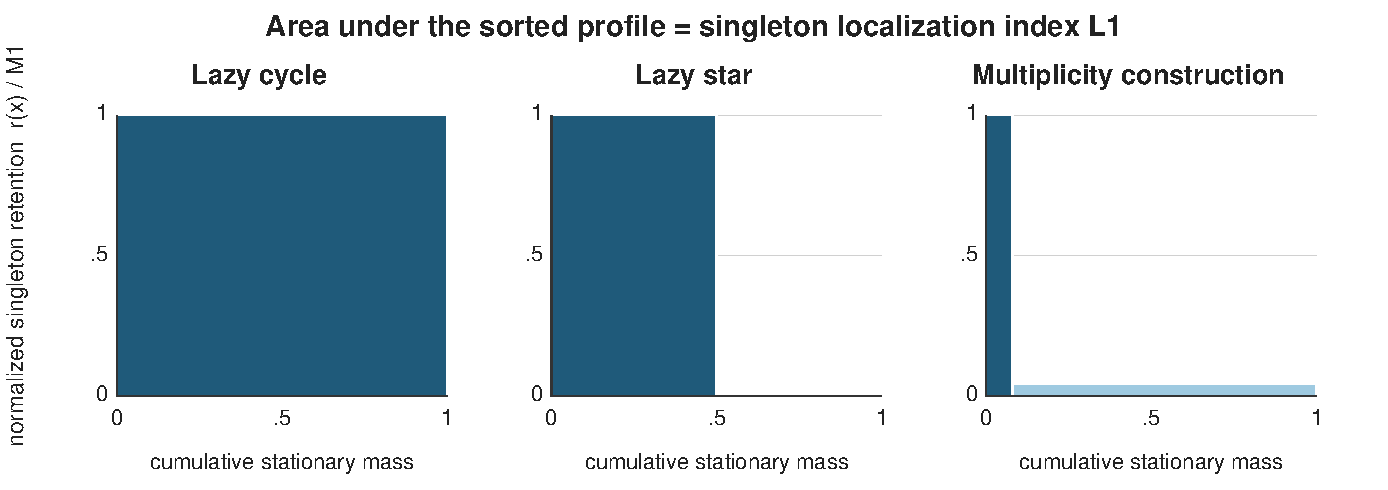
\includegraphics[width=\textwidth]{figures/singleton-retention-profiles.pdf}
  \caption{Decreasing rearrangements of the normalized singleton values
  \(r(x)/\Mone\), plotted against cumulative stationary mass.  These are
  profile plots rather than plots of the survival function \(F_1\); the area
  under each profile equals \(\Lone\).  The lazy cycle is homogeneous
  (\(\Lone=1\)), while the lazy star has a two-level profile
  (\(\Lone=1/2\)).  The third panel uses the finite multiplicity construction
  with
  \(\varepsilon=0.08\), \(k=256\), \(N=300\), and \(\delta=0.005\):
  \(\Lone=0.122\), while the set-conditioned witness satisfies
  \(R(A)=0.983\).  Thus a small singleton area can coexist with almost
  complete collective retention.}
  \label{fig:profiles}
\end{figure}


\section{Conclusion and open problems}
\label{sec:conclusion}

The singleton profile answers a legitimate but limited question: where do
the point-mass KL witnesses live under the stationary law?  Its survival
curve distinguishes a homogeneous obstruction from a thin high-retention
region, and its stationary numerator connects cleanly to mutual information
and spectral mass.

The profile does not answer the global variational question.  Multiplicity
inside an identical-row class can make \(\Lone\) and \(\Mone\) vanish while
\(\etaStat\) tends to one.  This is not a defect in the calculation; it is
the information-theoretic content of the Jensen gap.  A cloud of
indistinguishable states can retain what no one state appears to retain
after normalization.

Set-conditioned retention supplies a natural first collective layer.
It aggregates identical-row copies, preserves clone-saturated tests under
proportional splitting, and detects low-escape sets through an explicit
binary projection.  It remains incomplete: \(\Mset\) can be expensive to compute,
depends on the chosen state representation, and need not equal the supremum over
arbitrary tilted laws.

The most useful open problem is therefore structural rather than spectral.
Find verifiable row-separation conditions under which mutual information
dominates entropy inflation strongly enough to imply
\[
  \etaStat\le C\,\Mone
\]
with a dimension-free constant, or even
\(\etaStat=(1+o(1))\Mone\).  Natural candidates include lower bounds on
pairwise Jensen--Shannon or Hellinger separation, information radius,
and bounded-likelihood conditions coupled to the cardinality of
near-maximal row classes.

A second problem is to design a representation-stable hierarchy between
singletons and all input laws.  The clone-fiber identity in
Proposition~\ref{prop:splitting} is one exact datum, but arbitrary
refinements and quotient chains lose information in different ways.
A useful theory should state precisely which transformations it respects
and what computational price is paid at each collective level.


\appendix

\section{Supplementary spectral comparisons}
\label{app:spectral}

Throughout this appendix, \(P\) is reversible with respect to \(\pi\), with
eigenvalues as in Section~\ref{sec:spectral}.  Choose an orthonormal eigenbasis
\(\phi_1\equiv1,\phi_2,\ldots,\phi_n\) in
\(L^2(\pi)\), and write \(\pi_{\max}=\max_x\pi(x)\).  For probability laws
\(q\) and \(\pi\) with full-support \(\pi\), define
\[
  \chi^2(q\|\pi)
  :=\sum_y\frac{(q(y)-\pi(y))^2}{\pi(y)}.
\]

\begin{lemma}[\(\chi^2\)-spectral identity]
\label{lem:chi2}
For every \(x\in S\),
\[
  \chi^2(P(x,\cdot)\|\pi)
  =
  \sum_{i=2}^n\lambda_i^2\phi_i(x)^2.
\]
Consequently,
\[
  \sum_x\pi(x)\chi^2(P(x,\cdot)\|\pi)
  =\sum_{i=2}^n\lambda_i^2.
\]
\end{lemma}

\begin{proof}
The reversible spectral expansion is
\[
  \frac{P(x,y)}{\pi(y)}
  =
  \sum_{i=1}^n\lambda_i\phi_i(x)\phi_i(y).
\]
Subtract the \(i=1\) term, square, and average over \(y\sim\pi\).
Orthonormality gives the pointwise identity; averaging over \(x\) gives
the second.
\end{proof}

\begin{theorem}[Spectral comparison for stationary information]
\label{thm:spectral-comparison}
For every finite reversible chain,
\[
  J(P)\le\sum_{i=2}^n\lambda_i^2,
\]
and hence
\[
  \bar r_\pi
  \le
  \min\!\left\{
    1,\,
    \frac{\sum_{i=2}^n\lambda_i^2}
         {\log(1/\pi_{\max})}
  \right\}.
\]
If the likelihood ratios satisfy
\[
  \frac{P(x,y)}{\pi(y)}\le B<\infty
  \qquad(x,y\in S),
\]
then
\[
  c(B)\sum_{i=2}^n\lambda_i^2
  \le J(P)\le\sum_{i=2}^n\lambda_i^2,
\]
where
\[
  c(B):=
  \min_{0\le t\le B}
  \frac{t\log t-t+1}{(t-1)^2},
\]
with the continuous value \(1/2\) at \(t=1\).  For uniform \(\pi\), division
by \(\log n\) gives the corresponding bounds on \(\bar r_\pi\).
\end{theorem}

\begin{proof}
The inequality \(\KL(q\|p)\le\chi^2(q\|p)\), applied row by row and
combined with Lemma~\ref{lem:chi2}, gives the upper bound on \(J(P)\).
Moreover,
\[
  \bar r_\pi
  \le\frac{J(P)}{\log(1/\pi_{\max})},
\]
and independently \(\bar r_\pi\le1\).

For the lower bound, the defining quotient for \(c(B)\) extends to a
strictly positive continuous function on the compact interval \([0,B]\).
Thus, for \(0\le t\le B\),
\[
  t\log t-t+1\ge c(B)(t-1)^2.
\]
Apply this with \(t=P(x,y)/\pi(y)\), average first over \(y\sim\pi\) and
then over \(x\sim\pi\), and invoke Lemma~\ref{lem:chi2}.  This is the
standard functional-domination comparison between KL and \(\chi^2\);
see~\cite{SasonVerdu2016,NishiyamaSason2020}.
\end{proof}

\begin{remark}[Why the likelihood-ratio hypothesis matters]
For nonlazy simple random walk on a \(\Delta\)-regular graph with uniform
stationary law,
\[
  \max_{x,y}\left|\frac{P(x,y)}{\pi(y)}-1\right|
  =\max\{1,n/\Delta-1\}.
\]
The bounded-likelihood comparison is therefore not uniform for sparse
graphs.  In fact,
\[
  J(P)=\log(n/\Delta),
  \qquad
  \sum_{i=2}^n\lambda_i^2=\frac{n}{\Delta}-1,
\]
so their ratio tends to zero when \(\Delta\) is fixed.  The unconditional
spectral upper bound can also exceed one after normalization and is then
vacuous; this is why Theorem~\ref{thm:spectral-comparison} is explicitly
clipped at one.
\end{remark}

\subsection{Equal spectral gap, different singleton geometry}

\begin{proposition}[Three-state comparison]
\label{prop:same-gap}
Consider
\[
  P_A=
  \begin{pmatrix}
  0&1/2&1/2\\
  1/2&0&1/2\\
  1/2&1/2&0
  \end{pmatrix},
  \qquad
  P_B=
  \begin{pmatrix}
  1/2&1/4&1/4\\
  1/2&1/2&0\\
  1/2&0&1/2
  \end{pmatrix}.
\]
Both are reversible and have absolute spectral gap \(1/2\), but
\[
  \Lone(P_A)=1,\qquad \Lone(P_B)=\frac12.
\]
\end{proposition}

\begin{proof}
The stationary laws are
\(\pi_A=(1/3,1/3,1/3)\) and
\(\pi_B=(1/2,1/4,1/4)\).  The nontrivial spectra are
\(\{-1/2,-1/2\}\) and \(\{1/2,0\}\), respectively.  Every row of \(P_A\)
has retention \(\log(3/2)/\log3\).  For \(P_B\), the first row equals
\(\pi_B\), while
\[
  \KL(P_B(i,\cdot)\|\pi_B)=\frac12\log2,
  \qquad
  \log(1/\pi_B(i))=\log4
  \quad(i=1,2).
\]
Thus \(r_B(0)=0\), \(r_B(1)=r_B(2)=1/4\), and the two high-retention
states carry stationary mass \(1/2\).
\end{proof}

\section*{Declarations}

\paragraph{Funding.}
No external funding was received.

\paragraph{Competing interests.}
The author declares no competing interests.

\paragraph{Data and code availability.}
The figure is generated deterministically by the script
\path{scripts/generate_retention_profile_figure.py} from the closed-form
expressions displayed in the paper.  The companion script
\path{scripts/validate_retention_claims.py} checks a representative finite
counterexample matrix and its block formulas, numerically realizes the
diagonal parameter choices for \(m=3,\ldots,15\), verifies the stated
three-state eigenpairs and profile values, and samples the binary comparison
and uniform bottleneck simplification on finite grids.  These automated
checks are transcription and regression checks; they supplement, but do not
replace, the analytic proofs.  No empirical dataset is used.  Both scripts
are included in the submission source archive.  The manuscript makes no
optimizer-based claims.


\begin{thebibliography}{99}
\raggedright

\bibitem{AhlswedeGacs1976}
R.~Ahlswede and P.~G\'acs,
\emph{Spreading of sets in product spaces and hypercontraction of the
Markov operator},
Ann.\ Probab.\ \textbf{4} (1976), 925--939.

\bibitem{BanerjeeEtAl2005}
A.~Banerjee, S.~Merugu, I.~S.~Dhillon, and J.~Ghosh,
\emph{Clustering with Bregman divergences},
J.\ Mach.\ Learn.\ Res.\ \textbf{6} (2005), 1705--1749.

\bibitem{CaputoEtAl2025}
P.~Caputo, Z.~Chen, Y.~Gu, and Y.~Polyanskiy,
\emph{Entropy contractions in Markov chains: half-step, full-step and
continuous-time},
Electron.\ J.\ Probab.\ \textbf{30} (2025), 1--29;
doi:10.1214/25-EJP1372; arXiv:2409.07689.

\bibitem{ChoiHirdWang2025}
M.~C.~H.~Choi, M.~Hird, and Y.~Wang,
\emph{Improving the convergence of Markov chains via permutations and
projections},
Random Structures Algorithms \textbf{66} (2025), no.~4, e70016;
doi:10.1002/rsa.70016; arXiv:2411.08295.

\bibitem{CohenEtAl1993}
J.~E.~Cohen, Y.~Iwasa, G.~Rautu, M.~B.~Ruskai, E.~Seneta, and G.~Zbaganu,
\emph{Relative entropy under mappings by stochastic matrices},
Linear Algebra Appl.\ \textbf{179} (1993), 211--235.

\bibitem{CoverThomas2006}
T.~M.~Cover and J.~A.~Thomas,
\emph{Elements of Information Theory},
2nd ed., Wiley, 2006.

\bibitem{DaeijavadAsoodeh2026}
A.~Daeijavad and S.~Asoodeh,
\emph{Local and global contraction principles for MCMC mixing},
arXiv:2606.03033, 2026.

\bibitem{GeigerTemmel2014}
B.~C.~Geiger and C.~Temmel,
\emph{Lumpings of Markov chains, entropy rate preservation, and
higher-order lumpability},
J.\ Appl.\ Probab.\ \textbf{51} (2014), 1114--1132;
arXiv:1212.4375.

\bibitem{GuPolyanskiy2023}
Y.~Gu and Y.~Polyanskiy,
\emph{Non-linear log-Sobolev inequalities for the Potts semigroup and
applications to reconstruction problems},
Commun.\ Math.\ Phys.\ \textbf{404} (2023), 769--831;
doi:10.1007/s00220-023-04851-1; arXiv:2005.05444.

\bibitem{LawlerSokal1988}
G.~F.~Lawler and A.~D.~Sokal,
\emph{Bounds on the \(L^2\) spectrum for Markov chains and Markov
processes: a generalization of Cheeger's inequality},
Trans.\ Amer.\ Math.\ Soc.\ \textbf{309} (1988), 557--580.

\bibitem{LevinPeres2017}
D.~A.~Levin and Y.~Peres,
\emph{Markov Chains and Mixing Times},
2nd ed., Amer.\ Math.\ Soc., 2017.

\bibitem{Lin1991}
J.~Lin,
\emph{Divergence measures based on the Shannon entropy},
IEEE Trans.\ Inform.\ Theory \textbf{37} (1991), 145--151;
doi:10.1109/18.61115.

\bibitem{Montenegro2007}
R.~Montenegro,
\emph{Sharp edge, vertex, and mixed Cheeger type inequalities for finite
Markov kernels},
Electron.\ Commun.\ Probab.\ \textbf{12} (2007), 377--389;
doi:10.1214/ECP.v12-1269; arXiv:math/0606167.

\bibitem{MorrisPeres2005}
B.~Morris and Y.~Peres,
\emph{Evolving sets, mixing and heat kernel bounds},
Probab.\ Theory Related Fields \textbf{133} (2005), 245--266.

\bibitem{NishiyamaSason2020}
T.~Nishiyama and I.~Sason,
\emph{On relations between the relative entropy and
\(\chi^2\)-divergence, generalizations and applications},
Entropy \textbf{22} (2020), 563;
arXiv:2004.11197.

\bibitem{PolyanskiyWu2017}
Y.~Polyanskiy and Y.~Wu,
\emph{Strong data-processing inequalities for channels and Bayesian
networks},
in \emph{Convexity and Concentration}, IMA Volumes in Mathematics and its
Applications, vol.~161, Springer, 2017, pp.~211--249;
doi:10.1007/978-1-4939-7005-6\_7.

\bibitem{Raginsky2016}
M.~Raginsky,
\emph{Strong data processing inequalities and
\(\Phi\)-Sobolev inequalities for discrete channels},
IEEE Trans.\ Inform.\ Theory \textbf{62} (2016), 3355--3389;
doi:10.1109/TIT.2016.2549542; arXiv:1411.3575.

\bibitem{SasonVerdu2016}
I.~Sason and S.~Verd\'u,
\emph{\(f\)-divergence inequalities},
IEEE Trans.\ Inform.\ Theory \textbf{62} (2016), 5973--6006;
arXiv:1508.00335.

\end{thebibliography}

\end{document}
